
% Section: ARCHITECTURE

\subsection{Framework for Distributed Community Cloud System}
\label{sec:design-architecture}

%% >> Updated text copied from ComNet'15 paper
We foresee realising the community cloud by deploying a community cloud platform tailored to the specific infrastructure and context of community networks. A standard cloud platform is usually a centralised platform designed to perform resource management. There are quite a few well known cloud platforms for managing public and private clouds, like OpenStack \cite{OpenStack} and OpenNebula \cite{OpenNebula} among others. 
In our effort nevertheless, we focus on providing a framework that would allow users to share resources and access collaboratively-built services in a distributed manner.
For instance, a community cloud platform would require incentive mechanisms inspired by the social nature of community networks integrated into resource regulation components to encourage contribution from the members of the community network~\cite{Khan2015Incentive}.

\subsubsection{Layers of Community Cloud System}
We propose a framework that can serve as the core of a community cloud system. Our community cloud framework is a distributed bottom-up resource sharing and collaborative services platform.
This is achieved by adopting a layered architecture, as shown in Figure~\ref{fig:cloud-architecture}. 

\begin{figure}[tbp]
	\centering
	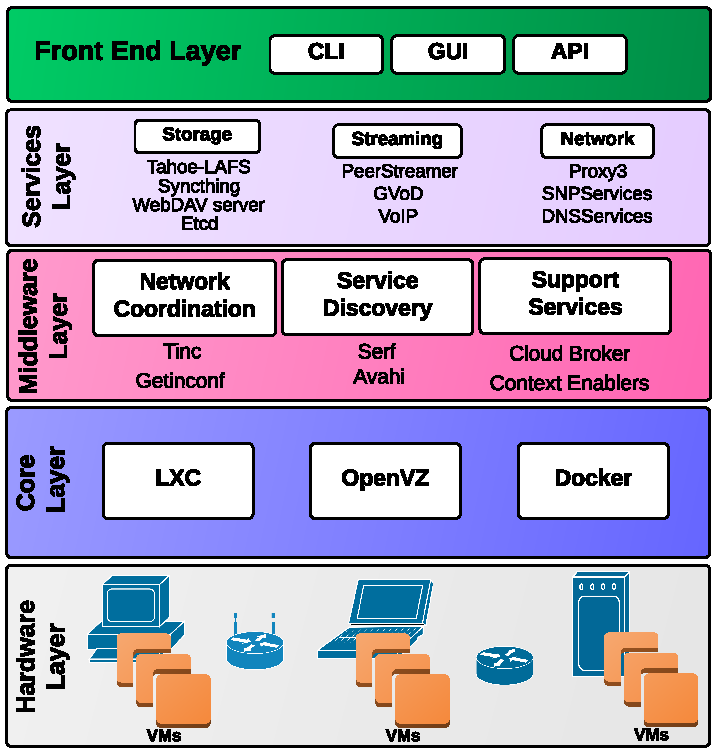
\includegraphics[width=0.6\textwidth,keepaspectratio]{ccarchitecture} 
	\caption{Framework for community cloud management system}
	\label{fig:cloud-architecture}
\end{figure}

\begin{enumerate}
	
	\item The \textbf{Hardware layer} provides the physical infrastructure needed to run the cloud services and applications. The hardware in the community networks customarily consists of SNs, client nodes, routers and the communication infrastructure, along with any computation, storage and other resources attached to the nodes.
	
	\item The \textbf{Core layer} is responsible for managing the hardware as virtualised resources. 
	It consists of components, such as a manager for the hosts and the network as well as a controller, scheduler, monitor, and data storage for virtual instances. 
	Many popular open-source software programs can be integrated to provide virtualisation, for instance LXC (Linux Containers) \cite{LXC}, OpenVZ \cite{OpenVZ}, and Docker \cite{Docker}, etc.

	\item The \textbf{Middleware layer} amalgamates the resources from multiple local community clouds, providing an integrated and consistent view of the cloud system to the cloud services. This requires a network coordination component to identify and manage different local clouds and a service discovery component to keep track of the services provided by the various clouds. Other support services can include:
	
	\begin{itemize}	
	\item Cloud coordinator and services broker components for assisting in combining resources from multiple cloud providers.
	\item Social and economic context enablers~\cite{Khan2014Architecture} that take advantage of the social and economic characteristics of the community networks to encourage participation from community network members and to ensure sustainability of the community cloud model.
	\item Incentive-based resource regulation and allocation mechanisms~\cite{Khan2015Incentive}.
	\item Trusted auctioneer~\cite{Khan2016Distributed} module for auction-based resource allocation schemes.
	\end{itemize}	 
	
	\item The \textbf{Services layer} integrates useful services and applications providing utilities for the community network members to encourage their participation. Common services include storage, video streaming, video on demand, voice over IP (VoIP), and network applications.
	
	\item The \textbf{Front-end layer} provides the interface to interact with the infrastructure of the community cloud, including command line interfaces (CLI), graphical user interfaces (GUI), 
API, and any other tools for assisting in the development of cloud services and applications.
	 
\end{enumerate}

%
%\section[Collaborative Distributed Architecture]{Collaborative Distributed Architecture for Community Cloud}
%\label{sec:design}
%
%
%%%
%\begin{figure}[tbp]
%   \centering
%  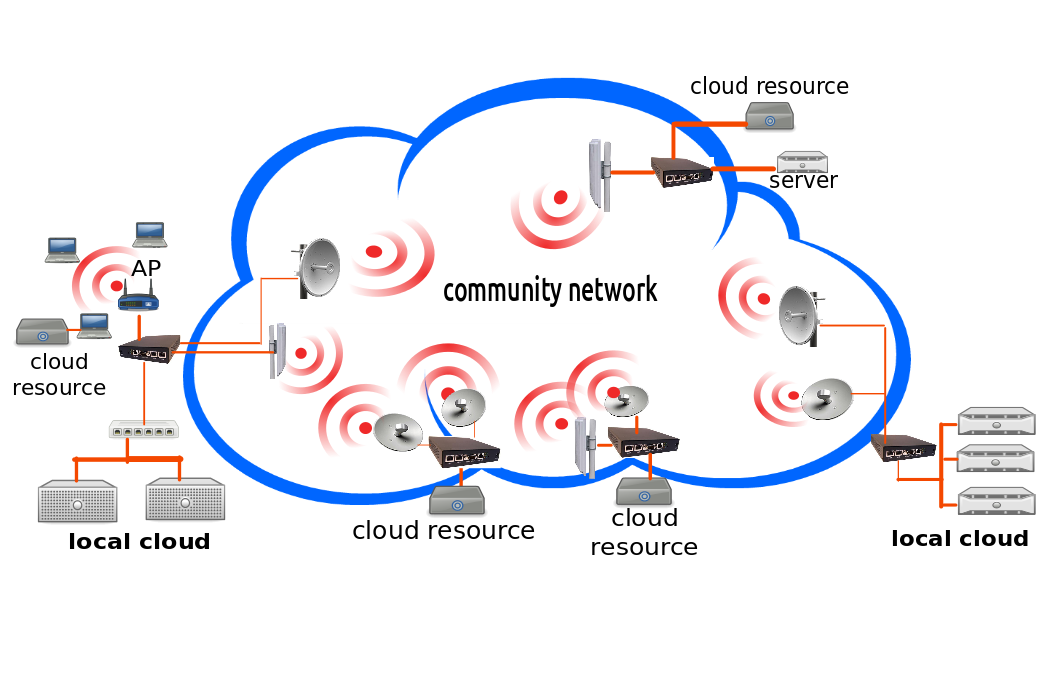
\includegraphics[width=2.85in,keepaspectratio]{com_node}
%   \caption{Nodes in a community network with cloud resources}
%   \label{fig:community-network}
%\end{figure} 
%
%
%A community network is managed and owned by the community, where nodes are managed independently by their owners. 
%The computer machines or nodes in a community network vary widely in their capacity, function and capability, as illustrated in Figure~\ref{fig:community-network}.
%Some hardware is used as super nodes (SNs) that have multiple wireless links and connect with other SNs to form the backbone of the community network, and are usually intended to be stable with permanent connectivity.
%Others act just as ordinary nodes (ON) and are only connected to the access point of a SN. 
%Topological analysis of the Guifi.net community network~\cite{Vega2012} indicates that from approximately 17,000 analysed nodes of Guifi.net, 7\% are SNs while the others are ONs.
%
%From the node types shown in Figure~\ref{fig:community-network}, it can be seen that principally the hardware for computation and storage is already available in community networks, consisting of some servers attached to the networking nodes. 
%No cloud services, however, are yet deployed in community networks to use this hardware as a cloud, leaving the community network services significantly behind the current standard of the Internet. 
%Our vision is that some community wireless routers will have cloud resources attached, building the infrastructure for a community cloud formed by several cloud resources attached to the nodes. 
%We note that ONs could principally also contribute cloud resources.
%
%%% Figure 
%\begin{figure}[tbp]
%   \centering
%   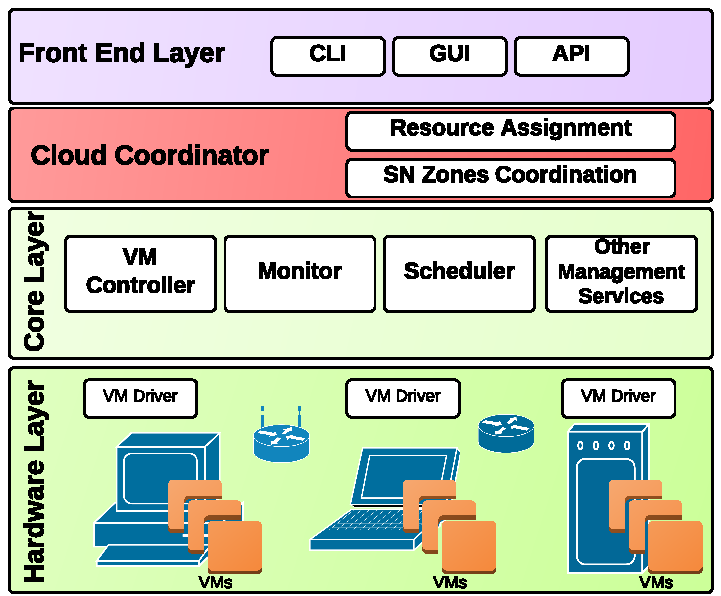
\includegraphics[width=3in,keepaspectratio]{vmm-architecture-generic}
%   \caption{Different layers of the community cloud management system}
%   \label{fig:overview-vmm-layers}
%\end{figure}
%
%An architecture for the community cloud system that manages such infrastructure needs to be robust, self-managing and efficient at handling the heterogeneity among the nodes. 
%The option for enabling a community cloud on which we focus here is to deploy a cloud management platform tailored to community networks on the nodes attached to the network. 
%There are a few cloud management systems available to manage public and private clouds, notably %
%    OpenStack\footnote{\url{http://www.openstack.org}}, 
%	OpenNebula\footnote{\url{http://www.opennebula.org}},
%	CloudStack\footnote{\url{http://cloudstack.apache.org}},
%	Eucalyptus\footnote{\url{http://www.eucalyptus.com}}
%	and Synnefo\footnote{\url{http://www.synnefo.org}}
%	among others.
%Such cloud management systems can be tailored for community networks by extending the existing functionality to address the particular conditions of community networks.
%For example, incentive mechanisms inspired by the social nature of community networks can be built into resource regulation component to encourage users to contribute resources~\cite{Khan2014Prototyping, Khan2013TowardsIncentives, Buyuksahin2013}. 
%    
%The conceptual overview for the cloud management system that we propose for community networks consists of multiple layers, as shown in Figure~\ref{fig:overview-vmm-layers}, with different components at each layer, as highlighted in Figure~\ref{fig:overview-vmm-hierarchy}.
%The nodes along with the communication infrastructure of the community network form the the hardware layer of the cloud architecture. 
%The core layer residing in the SN contains the software for managing and monitoring the virtual machines (VMs) on ONs.
%The front end layer provides the interface of the infrastructure service (Infrastructure-as-a-Service, IaaS).
%The components cloud coordinator, economic engine and social engine provide additional services for customising cloud infrastructure to the community networks, see Figure~\ref{fig:cloud-coordinator-components}. 
%
%%% Figure 
%\begin{figure}[tbp]
%   \centering
%   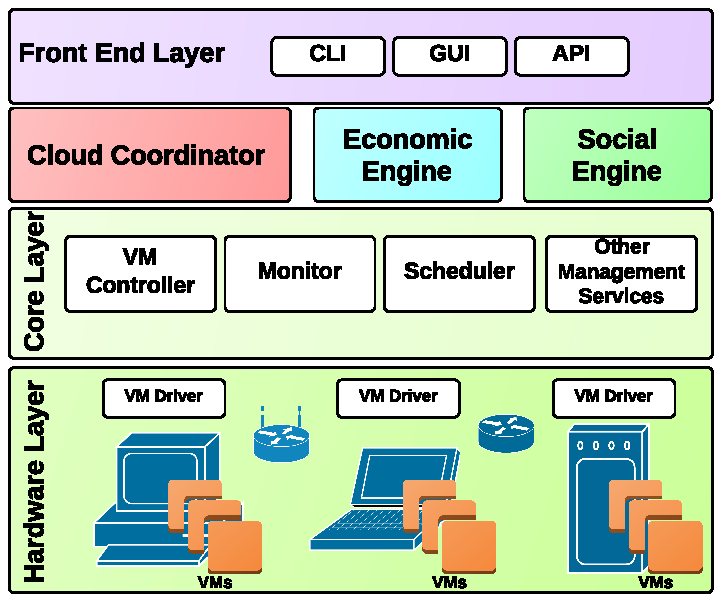
\includegraphics[width=3.1in,keepaspectratio]{vmm-architecture-generic-old} 
%   \caption{Architecture of the community cloud management system}
%   \label{fig:overview-vmm-hierarchy}
%\end{figure}
%
%
%The core of community cloud management system is the virtual machine manager (VMM) that is responsible for instantiating, scheduling and monitoring virtual machines on the nodes.
%The virtual machine manager consists of the following layers, which are common to most cloud computing architectures.
%
%
%\subsubsection{Hardware Layer}
%This consists of the physical infrastructure that is needed to run a cloud system. 
%The hardware in the community networks mostly consists of ONs and SNs and the wireless links provided by the mesh network, along with any attached computation, storage and other resources.
%
%\subsubsection{Core Layer}
%The core layer consists of components that are responsible for creation, allocation, scheduling, monitoring and management of VMs on the nodes. 
%This can include has following main components, some of which are shown in Figure~\ref{fig:overview-vmm-hierarchy}.
%    \begin{itemize}
%        \item Virtual Machines Controller
%        \item Virtual Machines Scheduler
%        \item Virtual Machines Monitor
%        \item Hosts Manager
%        \item Virtual Network Manager
%        \item Virtual Machines Image Data Store
%    \end{itemize}
%
%
%The functionality of the core layer is already provided by tools like OpenStack and others.
%Community cloud manager can, therefore, make use of these existing tools and extend their functionality to suit the needs of the community network.   
%
%
%\subsubsection{Cloud Coordinator} 
%The cloud coordinator is responsible for the federation of the cloud resources which are independently managed by different SNs.
%It provides the interface for other components like economic engine and social engine to request information from other SNs.
%The cloud coordinator components in different SNs connect among themselves in a decentralised manner to exchange relevant information about managing the available resources.
%By default applications running at a local cloud can only consume resources from the ONs directly managed by the local SN.
%With the cloud coordinator, the infrastructure service can provide a unified view of the resources contributed by multiple local clouds.
%When federating multiple local clouds, the cloud coordinator applies a peering regulation mechanism~\cite{Khan2014Prototyping, Khan2013TowardsIncentives} fed by the economic engine and social engine to perform resource allocation. 
%The cloud coordinator can consist of multiple components, some of which are indicated in Figure~\ref{fig:cloud-coordinator-components}.
%
%\begin{itemize}
%
%    \item Gossip-Based Discovery: 
%    The design of a community cloud manager follows a decentralised approach, so the cloud coordinator relies on gossip-based discovery mechanisms to manage overlay network of the SNs in community cloud.
%
%    \item Distributed Self-Management:
%    The community cloud has to efficiently manage the distributed resources in an autonomous way as ONs and SNs join and leave the network.
%    Distributed self-management forms a core component of the cloud coordinator to ensure successful operation of the community cloud.
%
%\end{itemize}
%
%
%%% Figure 
%\begin{figure}[tbp]
%   \centering
%   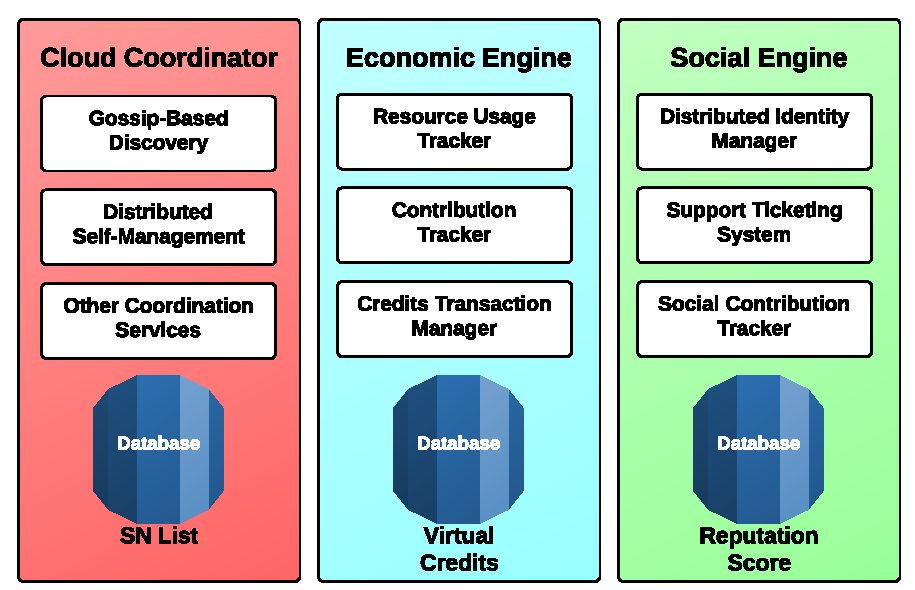
\includegraphics[width=3in,keepaspectratio]{vmm-architecture-detailed-old}
%   \caption{Distributed components of the community cloud management system}
%   \label{fig:cloud-coordinator-components}
%\end{figure}
%
%\subsubsection{Economic Engine}
%The role of economic engine is to manage the accounting and auditing for the infrastructure service so that the access can be regulated to the users of the community cloud.
%In contrast to public clouds, the main incentive for the providers in community clouds is the utility that they will get from the system by consuming its services and applications. 
%The economic engine manages a system of virtual credits that encourages the users to contribute resources to the cloud.
%This component will consist of many modules, some of which are highlighted in Figure~\ref{fig:cloud-coordinator-components}.
%
%\begin{itemize}
%
%    \item Resource Usage Tracker: 
%    This module connects with the VM Monitor in the core layer to get details about the resource usage.
%    It links this information to the user who requested the VMs and keeps record of it for accounting and auditing purposes.
%    This information forms the basis for regulating access to the resources.
%    
%    \item Contribution Tracker:  
%    The information from the VM Monitor is also fed to the contribution tracker module which uses it to register the resources     contributed by the owner of the nodes.
%    This information is used to reward the provider of the resources with virtual credits.
%        
%    \item Credits Transaction Manager:
%    This module manages the virtual credits database and credits or debits the account of different users with virtual credits.
%    The database gets updated whenever someone requests resources or contributes them to the community cloud.
%    The challenge for this module is to handle these transactions in a secure manner within a distributed system.    
%
%\end{itemize}
%
%\subsubsection{Social Engine}
%The community cloud is as much a social construct as it is a technical construct.
%The existence of the community cloud is not possible if there is a lack of participation from the community.
%Running a community cloud not only requires supply of technical resources like storage and network bandwidth, but also the time and effort of the users who setup and manage the network equipment. 
%Whereas the economic engine takes care of the incentives in the virtual world, the social engine is the component that encourages contribution in the physical world.
%We discuss here some of the modules that help to achieve this goal. 
%These modules may not be integral to the cloud management platform from a technical point of view, but nevertheless provide functionality necessary for the smooth running of the community cloud.
%
%\begin{itemize}
%
%    \item  Distributed Identity Manager: 
%    This module manages the global identity of the users in the system in a decentralised manner. %~\cite{Maler2008} 
%    This unique system-wide user ID is needed to track the usage and contribution by each user.
%
%    \item  Support Ticketing System:
%    This module provides a system for the users to help each other in resolving the problems encountered while using the community cloud.
%    The volunteers who provide the support to others are encouraged by rewarding them with better reputation in the system.
%    This reputation can then translate in to an increase in virtual credits which the user can spend for consuming services in the community cloud.
%
%    \item Social Contribution Tracker:
%    This module provides incentives to the volunteers who help with the smooth running of the community cloud.
%    The volunteers contribute with their time and effort to setup and maintain the hardware and network.
%    This module tracks this contribution of the volunteers in the reputation score database.
%    The social contribution tracker interacts with the credits transaction manager module in the economic engine and the users can exchange the reputation score with virtual credits.
%    The virtual credits allow the volunteers to consume the applications and services provided by the community cloud.
%
%\end{itemize}
%
%
%\subsubsection{Frontend Layer}
%The frontend layer provides the interface to interact with the infrastructure service of the community cloud. 
%This includes modules like command line interface (CLI), graphical user interface (GUI), application programming interface (API), and any other tools that assist with developing cloud application using the infrastructure service.    
% 
%
%\subsection{Interaction between Different Components} 
%
%We discuss here some usage scenarios and explain how different components of the community cloud management system can interact with each other.
%
%
%\subsubsection{Workflow for a resource request}
%Consider the case when a user requests a new VM from the community cloud. 
%The user connects to the GUI in the frontend layer and submits a request for a VM instance.
%The request is forwarded to the cloud coordinator that checks for availability at ONs, and if not available locally, forwards the request to neighbouring SNs.
%The cloud coordinator then checks with the identity manager component of the social engine, which authenticates the user to confirm whether the user has access to the resources.
%Cloud coordinator then checks the virtual credits database of the economic engine to see if the user has sufficient credits available to fulfil the request.
%After confirming that the user can consume resources, the request is forwarded to the scheduler in the core layer which selects the ON where the VM will run.
%The monitor in the core layer provides the details of the consumed resources to the resource usage tracker component in the economic engine.
%The credits transaction manager in the economic engine updates the credits of the requester and provider of the VM in virtual credits database.
%The contribution tracker in the economic engine updates the details for the provider.
%The user who requested the VM can check the GUI in the frontend layer for the status of the VM.
%
%
%\subsubsection{Workflow for social contribution}
%Consider the case when a user contributes to the community cloud by providing services like setting up routers or performing network maintenance.
%The user connects to a GUI application in the frontend layer and submits the details of her contribution. % separate GUI for different components?
%The request is forwarded to the cloud coordinator which contacts the identity manager and social contribution tracker components to confirm whether the user is registered, and also forwards the user's details to neighbouring SNs.
%The social contribution tracker updates the values for the user in the reputation score database.
%It also contacts the credits transaction manager component in the economic engine which updates the virtual credits database for the user.
%The social contribution tracker and the credits transaction manager provide the details to the frontend layer and the GUI informs the user of the outcome of the operation.
%
%
%\subsubsection{Workflow for support provision}
%Consider the case when a user contributes to the community cloud by providing support to others in resolving issues with the system.
%The support ticketing system in the social engine provides a mechanism for users to request and provide support on self-help basis.
%The main role of the support ticketing system in the community cloud is to provide incentives to the volunteers by rewarding them with virtual credits for their effort.
%When a user helps others with fixing their problems, the support ticketing system keeps track of the feedback.
%It checks with the identity manager component of the social engine to authenticate the user.
%The social contribution tracker then updates the reputation score database for the user, and also asks the credits transaction manager to update the virtual credits database for the user.
%The details are provided to the frontend layer where the user can see her virtual credits via the GUI. 

